% !TEX root = master_thesis.tex
\chapter{Experimental Setup}
\label{chap:exp}
In this work the beam asymmetry $\Sigma$ is determined in the reactions $\gamma p\to p\eta$ and $\gamma p\to p\eta'$, requiring a polarized photon beam and an unpolarized proton target. It is convenient to study photoproduction off a fixed target and investigate the resonances that occur in the process. The analyzed data was taken at the CBELSA/TAPS experiment located in Bonn  at the ELectron Stretcher Accelerator (ELSA). In this chapter the different parts of the CBELSA/TAPS experiment that are used for the measurement of the beam asymmetry $\Sigma$ will be presented. 

High energy electrons extracted from ELSA are used to produce a polarized photon beam using the \emph{bremsstrahlung} process (see \ref{subsec:goni}). After they have been energy tagged (see \ref{subsec:tag}) these photons then interact with the fixed target material (see Section \ref{sec:tar}) so that hadronic resonances may be excited that will decay via the strong interaction under the emission of mesons. The resulting decay products can then be measured with a system of electromagnetic calorimeters and scintillators that is especially suited for the detection of photons (see Section \ref{sec:cal}). The analogue measurements are only saved for offline analysis if detector signals meet certain trigger conditions which is only the case for reactions that are of interest (see Section \ref{sec:trig}). This way the amount of unwanted background is minimized already during the process of data taking. Once data acquisition is finished the data may be investigated with the help of analysis software and Monte Carlo simulations (see Section \ref{sec:mc}) tailored to the needs of the CBELSA/TAPS experiment.
\section{Production of polarized high energy photon beam}
\label{sec:pol}
To measure polarization observables in photoproduction reactions a polarized photon beam is needed which can be created using \emph{coherent bremsstrahlung}. Bremsstrahlung is the dominating interaction of high energy ($\mathcal{O}\left(\SI{1e0}{\giga\eV}\right)$) electrons with matter \cite{leo}. Electrons are decelerated in the \textsc{Coloumb} field of heavy nuclei and radiate real photons. To conserve momentum there has to be a momentum transfer $q$ which is negligibly small compared to the nucleon mass. If an amorphous radiator is used incoherent bremsstrahlung is produced with a continuous spectral distribution proportional to $1/E_\gamma$ according to the \textsc{Bethe-Heithler} cross section \cite{hei}. Since the structure of nuclei in the amorphous radiator does not exhibit any periodicity, the electric field vector will not prefer any particular direction, resulting in a net polarization degree of zero for the photon beam. To achieve non-vanishing polarization degrees a crystal with periodic placement of nuclei may be used as radiator. Then, coherent bremsstrahlung is produced; the crystal can absorb the recoil only for discrete momenta $q_n$ meeting the \textsc{Laue} condition of the crystal lattice. This enables constructive interference between different bremsstrahl photons and at the same time fixes the deflection plane of incoming electrons, resulting in a coherent polarized photon beam. Incoherent bremsstrahlung may still occur due to impurities in the crystal structure, so that the total bremsstrahlung cross section off a crystal radiator $\sigma_\text{crystal}$ is the sum of a coherent ($\sigma_\text{coherent}$) and an incoherent ($\sigma_\text{incoherent}$) part
\begin{equation}
	\sigma_\text{crystal}=\sigma_\text{coherent}+\sigma_\text{incoherent}.
\end{equation}
The process of bremsstrahlung can be modeled using ANalytical Bremsstarhlung (ANB) calculations \cite{anb}. ANB intensity spectra for a crystal and amorphous radiator are shown in Figure \ref{fig:anb} on the left hand side. The right hand side shows the enhancement spectrum, which is given by dividing the two spectra. 
\begin{figure}[htbp]
	\centering
	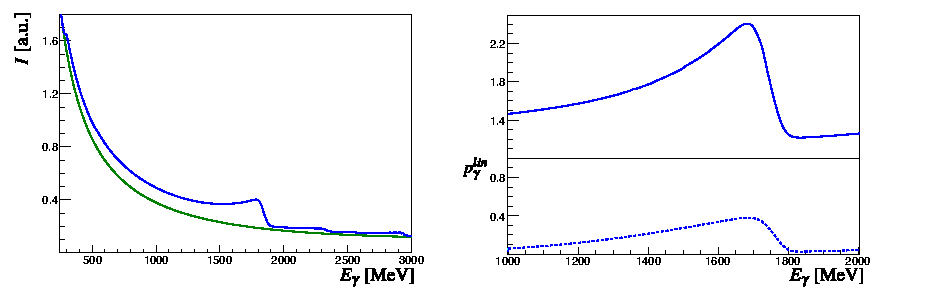
\includegraphics[width=\linewidth]{figs/anb.pdf}
	\caption{Left: Incoherent (green) and crystal (blue) bremsstrahlung intensities as a function of the photon energy. Right: The enhancement spectrum is given as the ratio of crystal to incoherent intensity spectrum. The dashed line at the bottom shows the calculated polarization degree. Both spectra are generated using ANB calculations. Taken from \cite{farahphd}.}
	\label{fig:anb}
\end{figure} 
One observes that the bremsstrahlung intensity spectrum obtained from a crystal radiator is in general enhanced relative to the incoherent spectrum obtained from an amorphous radiator. In fact, using ANB calculations, the polarization degree can be determined from the enhancement spectrum. The characteristic drop in intensity in the intensity spectrum obtained from the crystal radiator is referred to as the coherent edge. It occurs because the photon energy in the kinematically allowed region of the recoil momentum that will lead to coherent bremsstrahlung is limited. The relative alignment of the radiation crystal to the electron beam determines the position of the coherent edge. 
\subsection{Goniometer}
To determine the beam polarization, spectra from a diamond radiator as well as from an amorphous radiator are required. Several radiators are placed inside of the goniometer, see Figure \ref{fig:goni.}
\label{subsec:goni}
\begin{figure}[htbp]
	\centering
	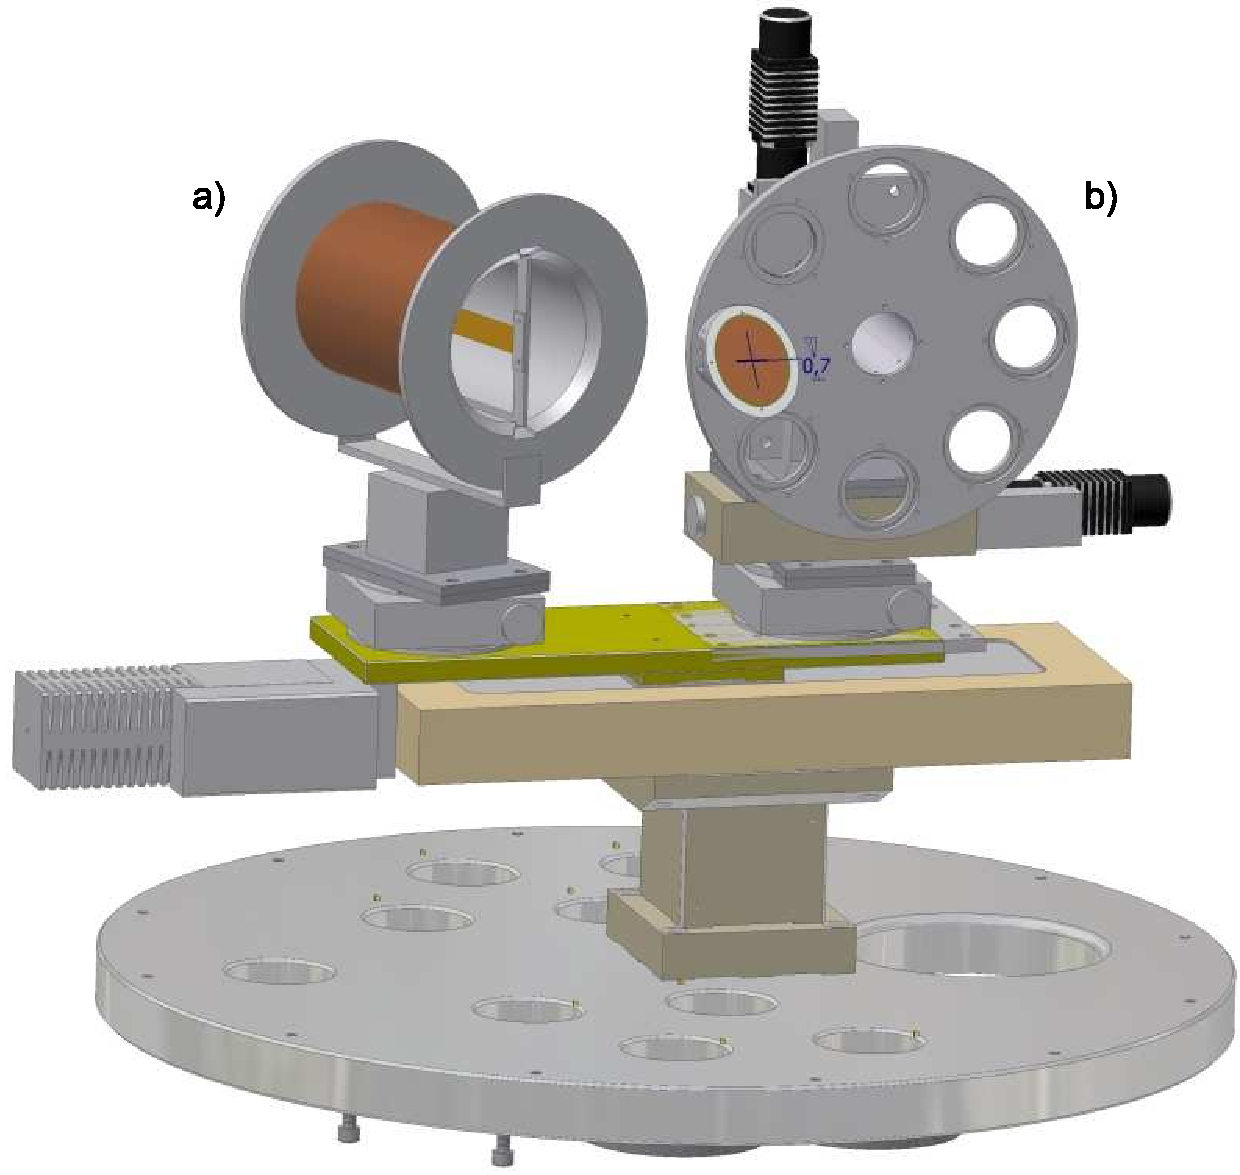
\includegraphics[width=.49\linewidth]{figs/goni-ganz.pdf}
	\caption{\cite{cb}}
	\label{fig:goni}
\end{figure}
\subsection{Tagging system}
\label{subsec:tag}
\begin{figure}[htbp]
	\centering
	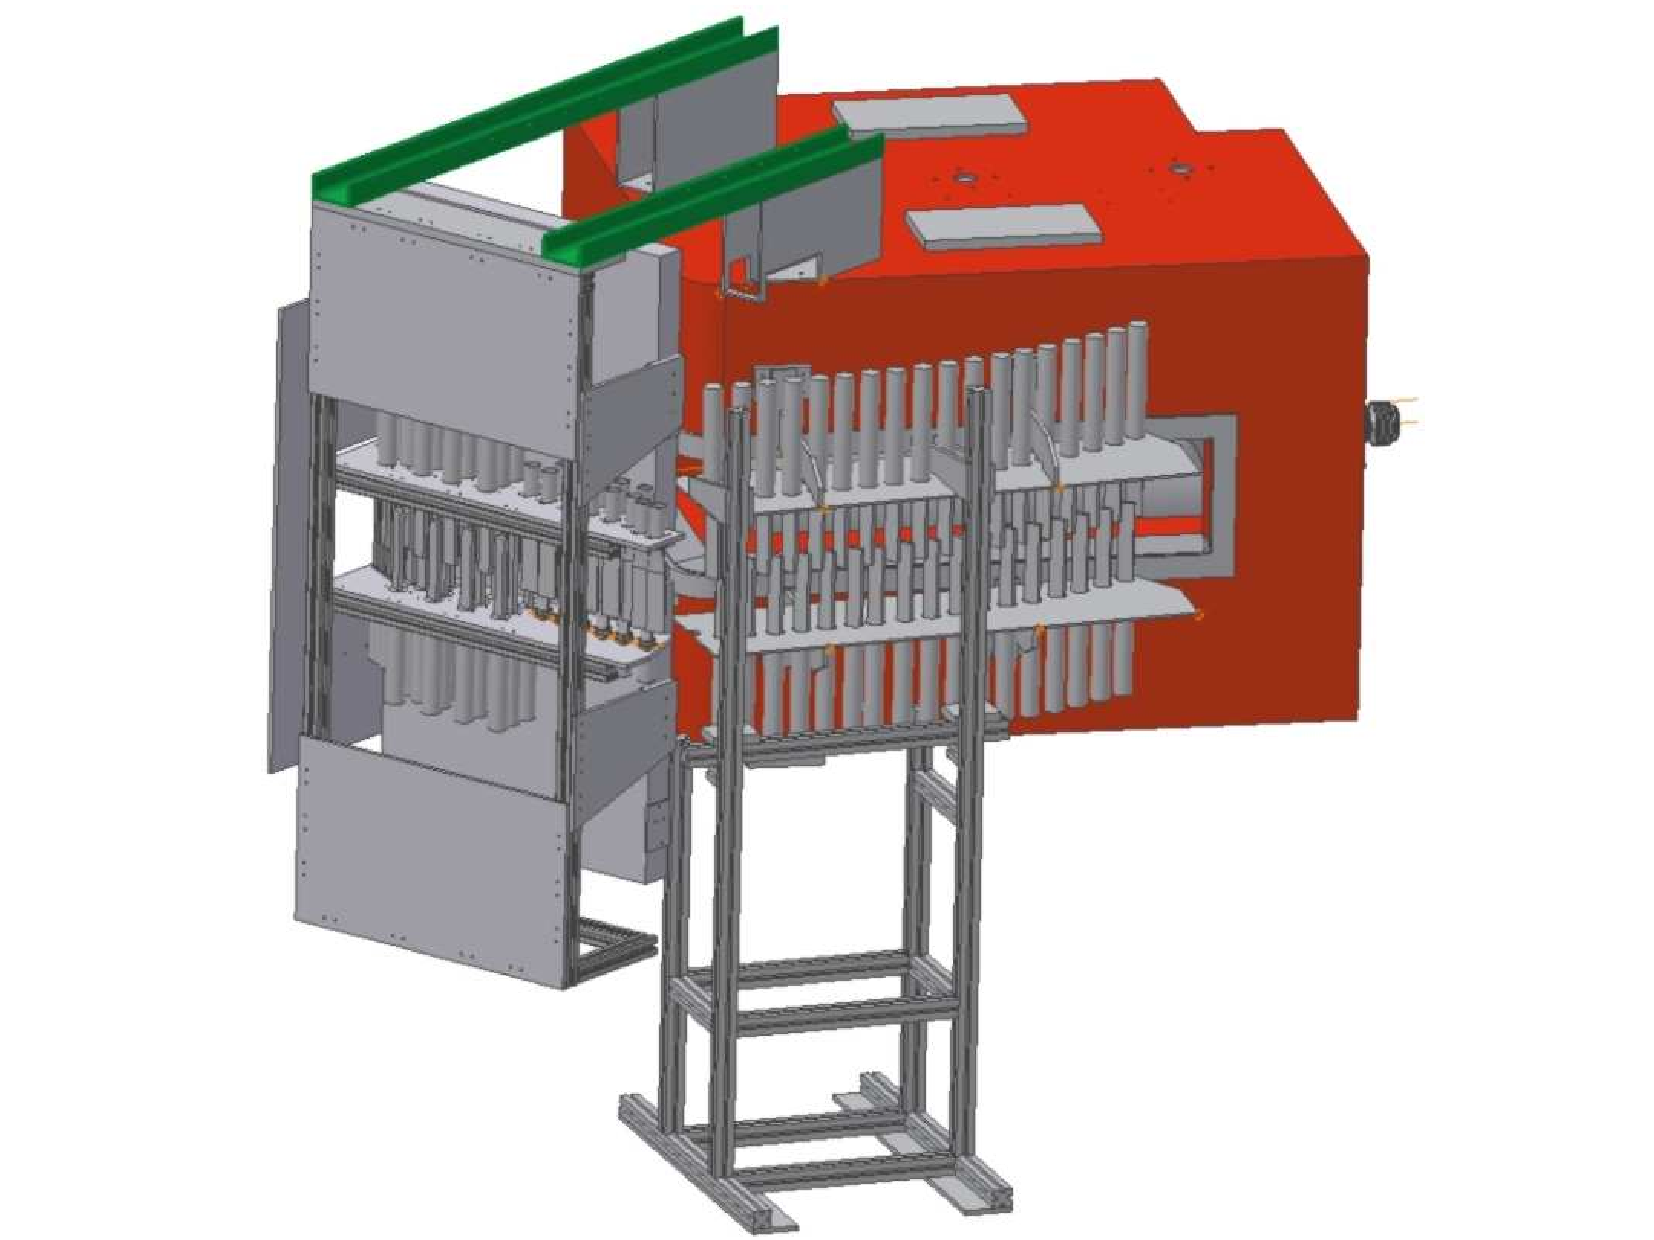
\includegraphics[width=.49\linewidth]{figs/Tagger.pdf}
	\caption{\cite{cb}}
\end{figure}
\section{Liquid hydrogen target}
\label{sec:tar}
\begin{figure}[htbp]
	\centering
	\includegraphics[width=.5\linewidth]{figs/Target.pdf}
	\caption{\cite{cb}}
\end{figure}

\section{Calorimeters}
\label{sec:cal}
\begin{figure}[htbp]
	\centering
	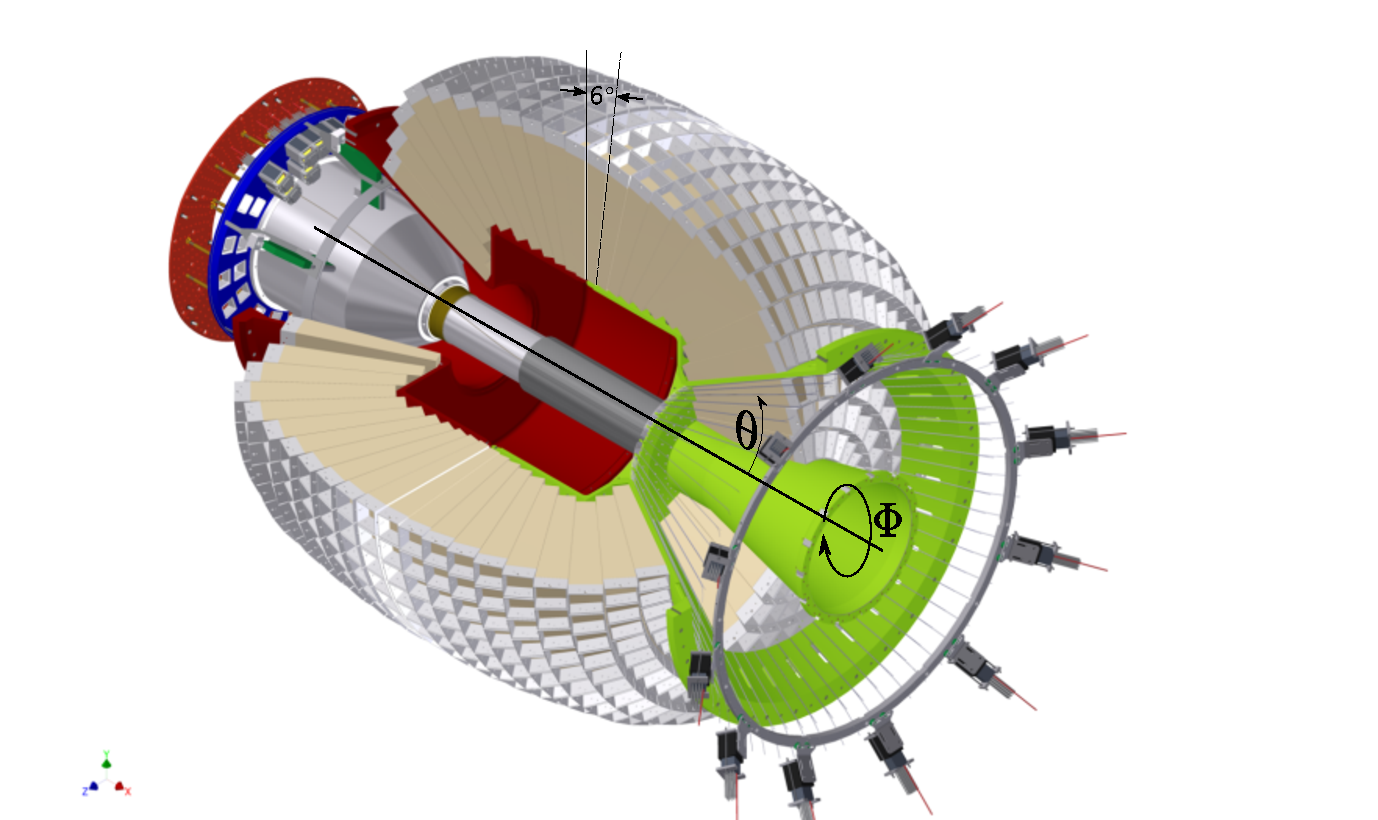
\includegraphics[width=\linewidth]{figs/cb_fp_in.pdf}
	\caption{\textsc{D. Walther} in \cite{urban}}
\end{figure}
\begin{figure}[htbp]
	\centering
	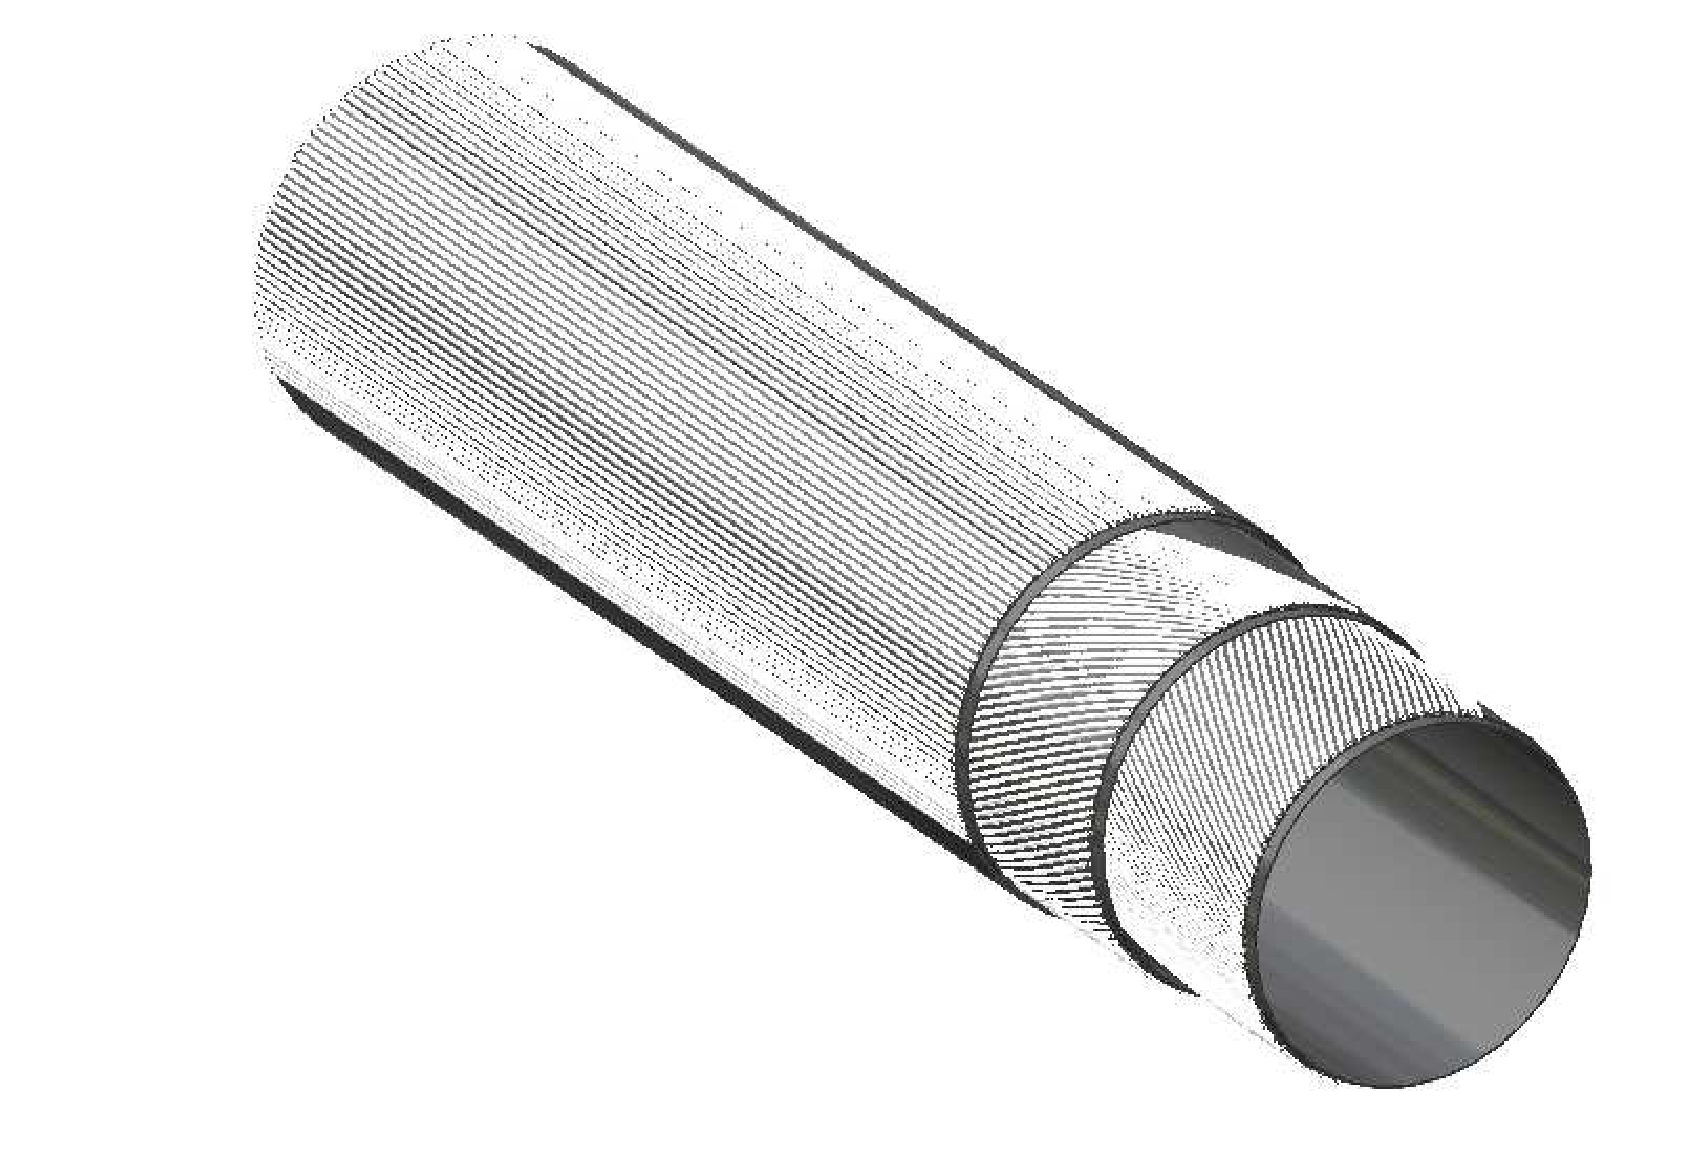
\includegraphics[width=.5\linewidth]{figs/faserorient.pdf}
	\caption{\cite{cb}}
\end{figure}
\begin{figure}[htbp]
	\centering
	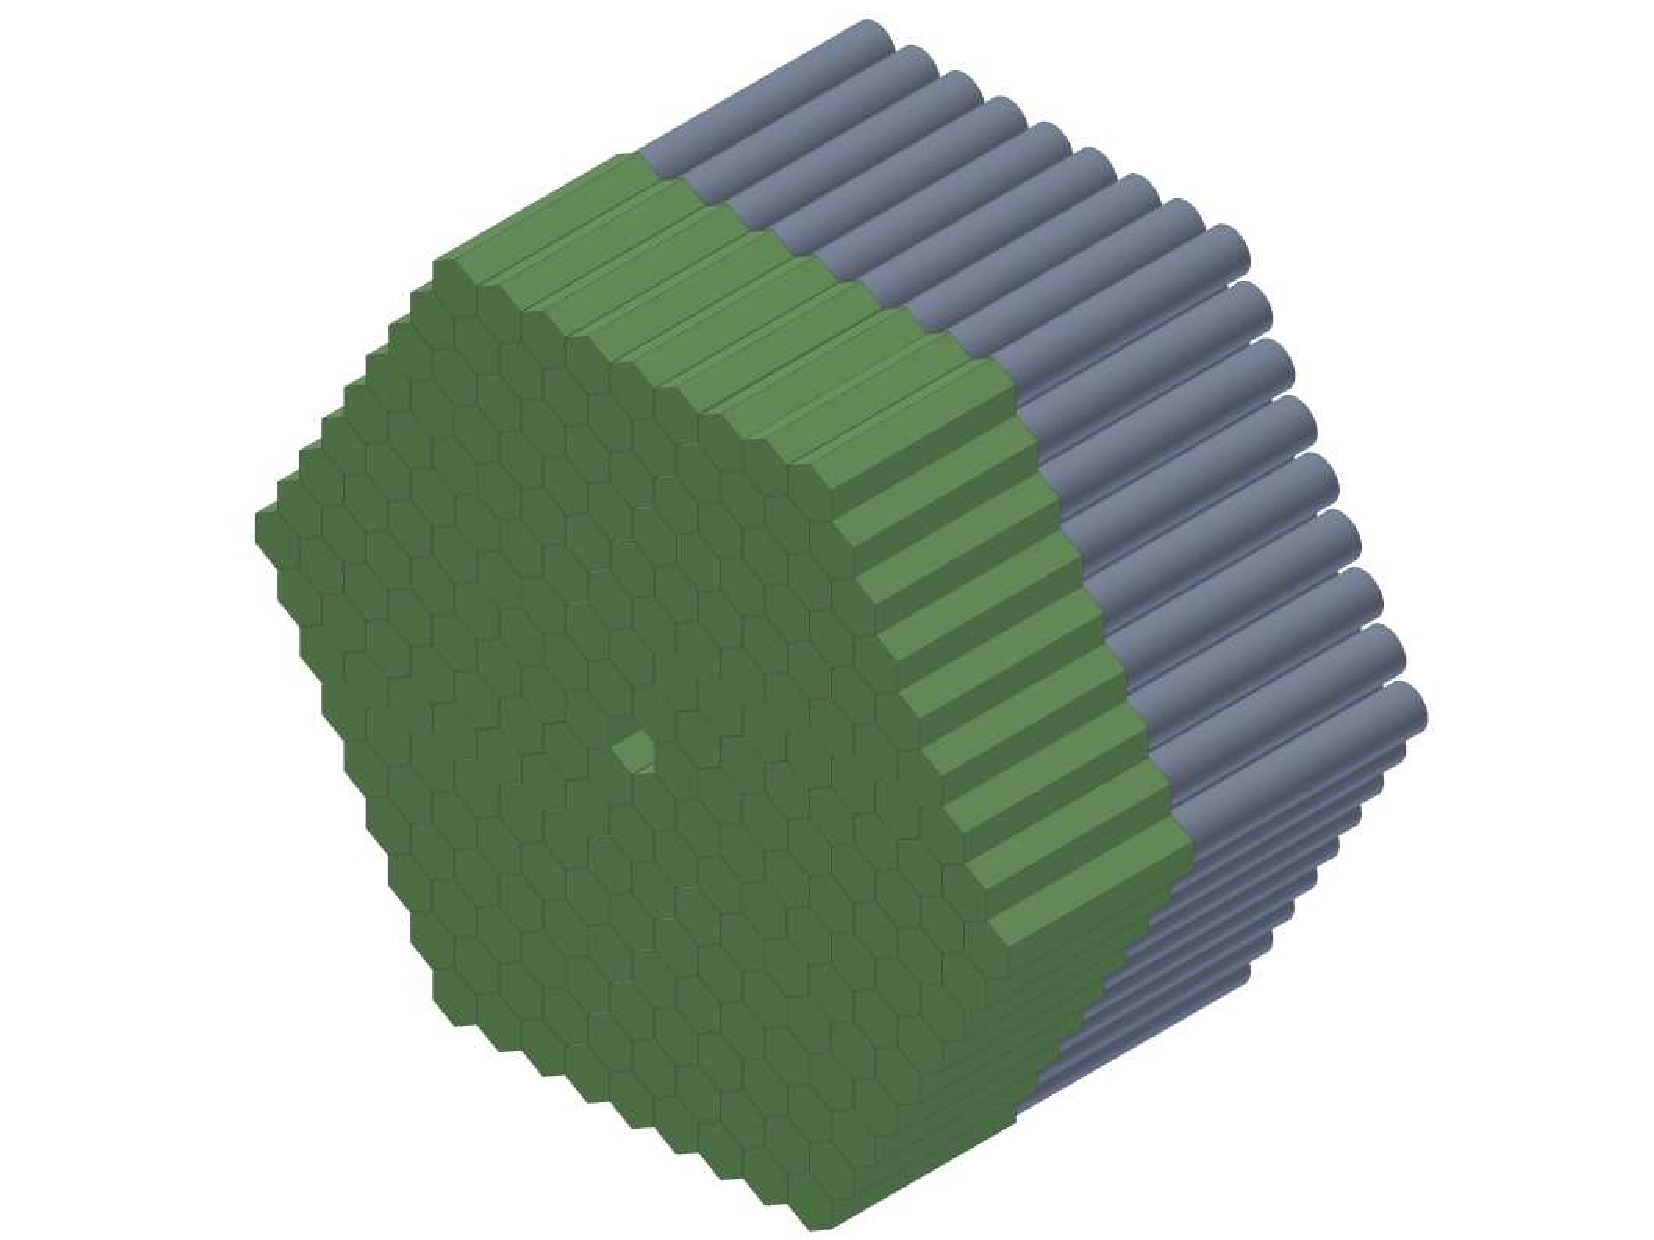
\includegraphics[width=.5\linewidth]{figs/mini-taps.pdf}
	\caption{\cite{cb}}
\end{figure}

\section{Trigger}
\label{sec:trig}

\section{Software and Monte Carlo}
\label{sec:mc}
\section{Datasets}